%%%%%%%%%%%%%%%%%%%%%%%%%%%%%%%%%%%%%%%%%%%%%%%%%%%%%%%%%%%%%%%
%         Estudio empírico de las funciones de activación
%%%%%%
%   1. Comparativas en cuanto a coste computacional.
%%%%%%%%%%%%%%%%%%%%%%%%%%%%%%%%%%%%%%%%%%%%%%%%%%%%%%%%%%%%%%%

\chapter{Funciones de activación}

Como se observó en 
% TODO referencia a que no hay idoneidad a nivel teórico 
% sobre una función de 
se desconoce teóricamente si una función de activación va a ser 
mejor que otra, es por ello y puesto que nuestro objetivo 
es reducir el coste computacional de una red neuronal
que procederemos a realizar un análisis del costo de las redes neuronales. 


\section{Caracterización de las funciones de activación}  

Si bien por conveniencia teórica definimos las funciones de activación en \ref{def:funcion_activacion_articulo}
como una función de $\phi:\R \longrightarrow [0,1]$, no 
decreciente, con uno como límite en infinito y cero como límite a 
menos infinito. 

Nos basaremos en el concepto actual de función de activación,
basta con que sea una función no polinómica
(véanse  los artículos \cite{DBLP:journals/corr/SonodaM15}, \cite{modern-trainable-activation-functions} y \cite{FUNAHASHI1989183}),
además también incluiremos la función de activación identidad.

Funciones no polinómicas hay infinitas y reincidimos en que a priori no hay una mejor que otra; por tanto, como criterio de selección nos guiaremos por la intuición que nos brinda la demostración del teorema \ref{teorema:2_3_uniformemente_denso_compactos}.
  La imagen de una función de activación es relevante a la hora de aproximar la función ideal desconocida, ya que reduce el número 
  de neuronas si se usa convenientemente.  
Por lo tanto una buena heurística sería disponer de un repertorio básico de funciones de activación que contemplen distintas imágenes no polinómicas. 

Además de las propuestas en \ref{def:funcion_activacion_articulo}, 
añadimos a nuestra colección las siguientes. 

\begin{table}[H] 
    \centering  
    \begin{tabular}{| c | c | c | c |}
        \hline
        Nombre & Expresión & Rango imagen  & Gráfica \\
        \hline
        %%%%%%%% Identidad %%%%%%%
        % Nombre: 
        Identidad 
        & %expresión 
        $Id(x) = x$
        & % Rango imagen
        $(-\infty, +\infty)$
        & % Gráfica
        \begin{minipage}{.4\textwidth}
            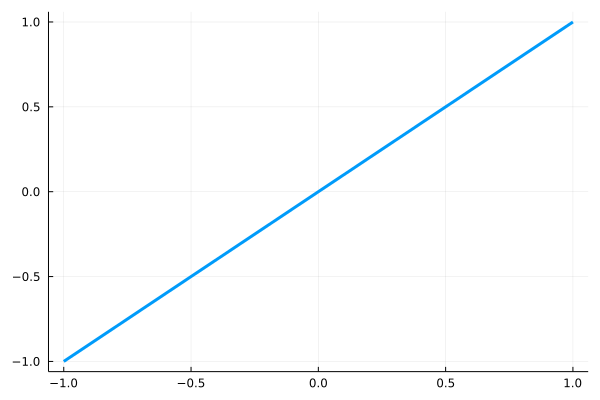
\includegraphics[width=\linewidth]{funciones-activacion/Identidad.png}
        \end{minipage}
        \\
        \hline
        %%%%%%%% sigmoide %%%%%%%%
        % Nombre: 
        Sigmoidea 
        & %expresión 
        $\sigma(x) = \frac{1}{1+e^{-a}}$
        & %Rango imagen
        $(0,1)$
        \\
        \hline
        %%%%%%%% sigmoide  bipolar %%%%%%%%
        % Nombre: 
        Sigmoide bipolar 
        & %expresión 
        $\sigma(x) = \frac{1+e^{-a}}{1+e^{-a}}$
        &% Rango imagen
        $(-1,1)$
        \\
        \hline
        %%%%%%%% Tangente hiperbólica  %%%%%%%%
        % Nombre: 
        Sigmoide bipolar 
        & %expresión 
        $\tanh$
        & %Rango imagen
        $(-1,1)$
        \\
        \hline
        %%%%%%%% Valor absoluto%%%%%%%%
        % Nombre: 
        Valor absoluto
        & %expresión 
        $abs(x)= |a|$
        & Rango imagen
        $[0,+\infty]$
        \\
        \hline
         %%%%%%%% Coseno %%%%%%%%
        % Nombre: 
        coseno
        & %expresión 
        $\cos$
        & %Rango imagen
        $[-1,1]$
        \\
        \hline
        %%%%%%%% ReLU %%%%%%%%
        % Nombre: 
        ReLU
        & %expresión 
        $ReLu(x) = \max(0,x)$
        & %Rango imagen
        $[0,+\infty)$
        \\
        \hline
    \end{tabular}
    \caption{Compendio de funciones de activación}  
    \label{table:funciones-de-activation}
\end{table}


